\chapter{Hyperspherical Coordinates}
This appendix contains mapping procedures, derivations and implementation details for \Cref{chap:4}. Some of the definitions presented in \cref{MNJC} will be repeated here in order for this appendix to be complete.

\section{Mass Normalized Jacobi Coordinates}
Prior to the introduction of either non-symmetric or symmetric coordinates  we introduce a set of mass normalized Jacobi coordinates, which will be used in combination with both Delves and modified Smith--Whitten coordinates. 

Let $\mathbf{x}_i$ and $m_{i}$ be the position vector and mass of the $i$th particle in the laboratory frame. If the total mass $M$, the three particle reduced mass $\mu$, and the normalizing constants $d_{k}$ $(k=1,2,3)$ are given by

\begin{align}
M &= \sum_{i=1}^{3}m_i, \\
\mu^2 &= \frac{1}{M}\prod_{i=1}^{3}m_i,\\
d_k^2 &= \frac{m_k}{\mu}\frac{(m_i+m_j)}{M},
\end{align}
then the set of mass-scaled Jacobi vectors and the centre-of-mass coordinate can be defined as

\begin{align}
\mathbf{r}_k &= d^{-1}_k(\mathbf{x}_{j}-\mathbf{x}_{i}), \label{eq:app_jacobi1} \\
\mathbf{R}_k &= d_k\Big[\mathbf{x}_{k}-\frac{(m_{i}\mathbf{x}_{i}+m_{j}\mathbf{x}_{j})}{m_{i}+m_{j}}\Big], \label{eq:app_jacobi2}\\
\mathbf{X}_{CM} &= \frac{1}{M} \sum_{i=1}^{3} m_{i} \mathbf{x}_{i},
\end{align}   
in which, the indices $i,j,k$ are cyclic permutations of $(1,2,3)$. The centre-of-mass is separated out and will not be considered further. Transformations within the set of coordinates is aided by defining the angle $\beta_{ij}$, which has the following properties

\begin{subequations}
	\begin{align}
	&\beta_{ij} = -\beta_{ji}, \quad \beta_{ii} = 0,\\
	&\tan\beta_{ij} = -m_k/\mu,\\
	&d_{i}d_{j} \sin\beta_{ij} = 1,\\
	&d_{i}d_{j} m_{k} \cos\beta_{ij} = -\mu,\\
	&\beta_{12}+\beta_{23}+\beta_{31} = 2\pi.
	\end{align}
\end{subequations}
Orthogonal transformations are then given by 

\begin{equation}\label{eq:kinematic_rot}
\begin{pmatrix}
\mathbf{r}_j\\
\mathbf{R}_j
\end{pmatrix}
=
\begin{pmatrix}
\cos\beta_{ij} & \sin\beta_{ij}\\
-\sin\beta_{ij} & \cos\beta_{ij}
\end{pmatrix}
\begin{pmatrix}
\mathbf{r}_i\\
\mathbf{R}_i
\end{pmatrix}.
\end{equation}   

In the following sections I will introduce two of the most commonly used hyperspherical coordinates. The general idea is to combine the two Jacobi vectors into a single six-dimensional position vector $\mathbf{q}$, which represents a point in $\mathbb{R}^6$. The polar coordinates of this point are given by the hyperradius $\rho$ and five hyperangles $\Omega$. The hyperradial coordinate is both rotationally and permutationally invariant and is, regardless of the specific choice of $\Omega$, defined by

\begin{equation}\label{eq:hyperradius}
\rho = \sqrt{\mathbf{r}^2 + \mathbf{R}^2}.
\end{equation}

\section{Delves Coordinates}\label{delves}
This section contains the detailed derivation of the three-body Schr{\"o}dinger equation written in Delves coordinates. To introduce Delves hyperspherical coordinates, we use the Jacobi vectors defined in \cref{eq:app_jacobi1,eq:app_jacobi2} and define Delves' hyperangle $\alpha_{k}$ as the polar angle of the position vector in the $(r_k,R_k)$ plane, i.e., 

\begin{equation}
\alpha_{k} = \arctan\bigg(\frac{r_{k}}{R_{k}}\bigg), \quad 0\leq \alpha_{k} \leq \frac{\pi}{2}.
\end{equation}
This angle together with \Cref{eq:hyperradius} is then used to map the Jacobi coordinates to a point on the plane in hyperpolar space through 

\begin{subequations}
	\begin{align}
	r_{k} &= \rho \sin{\alpha_{k}},\\
	R_{k} &= \rho \cos{\alpha_{k}}.
	\end{align}
\end{subequations}

The four remaining angles can be defined as the spherical angles of $\mathbf{r}_k$ and $\mathbf{R}_k$, which is suitable if we work in the laboratory-frame. However, we are interested in the body-fixed frame and then it is better to instead define three of these angles as the external Euler angles and the fourth angle as the angle between the two vectors $\mathbf{r}_{k}$ and $\mathbf{R}_{k}$, which is given by

\begin{equation}
\cos{\theta_{k}} = \frac{\mathbf{r}_{k} \cdot \mathbf{R}_{k}}{r_{k} R_{k}}, \quad  0\leq \theta \leq \pi.
\end{equation}

We chose one arbitary set to work in and suppress the indices from hereon. The mass weighted Schr{\"o}dinger equation for the stationary wavefunction $\Psi$ of a three-body system, with position vectors $\mathbf{x}_i$ and masses $m_i$, ($i=1,2,3$), interacting pairwise through a potential $V$, is given by

\begin{equation}
-\frac{1}{2} \sum_{i=1}^{3} m^{-1}_{i} \nabla^{2}_i \Psi + V\Psi = E \Psi. 
\end{equation}
Where $\nabla_i^{2}$ is the Laplace operator for particle $i$, which in spherical coordinates reads

\begin{equation}
\nabla_i^2 = \frac{1}{r_i^{2}}\frac{\partial}{\partial r_i} \bigg(r_i^{2} \frac{\partial}{\partial r_i}\bigg) - \frac{L_i^{2}}{r_i^{2}},
\end{equation}
in which $L_i$ is the angular momentum operator associated with the vector $\mathbf{r}_i$. 

The kinetic energy for three particles in the mass normalized Jacobi coordinates was given in \Cref{eq:6}. Thus, after separating out the centre-of-mass coordinate, the Schr{\"o}dinger equation for the internal motion is simply 

\begin{equation}
-\frac{1}{2\mu} \bigg(\nabla^{2}_{\mathbf{r}} + \nabla^{2}_{\mathbf{R}}\bigg) \Psi + V\Psi = E \Psi. 
\end{equation}

For three identical particles, the squared orbital angular momentum operators associated with the Jacobi vectors are given by  

\begin{equation}
L^{2}_r = L^{2}_{R} = -\frac{1}{\sin{\theta}} \frac{\partial}{\partial{\theta}} \bigg( \sin{\theta} \frac{\partial}{\partial{\theta}} \bigg).
\end{equation}
Change of coordinates subsequently results in the following transformations for the partial derivatives of the vector $\mathbf{r}$

\begin{align}
	\frac{\partial}{\partial r}  &= \frac{1}{\rho}\cos{\alpha}\frac{\partial}{\partial \alpha} + \sin{\alpha}\frac{\partial}{\partial \rho}, \\
	\frac{\partial^2}{\partial r^2} &=\frac{1}{\rho^2} \cos^2\alpha \frac{\partial^2}{\partial\alpha^{2}} - \frac{1}{\rho^2} \sin 2\alpha \frac{\partial}{\partial\alpha} + \sin^2\alpha \frac{\partial^2}{\partial\rho^{2}} \nonumber \\
	&+ \frac{1}{\rho} \cos^2\alpha \frac{\partial}{\partial\rho} + \frac{1}{\rho} \sin 2\alpha \frac{\partial^2}{\partial\alpha \partial\rho}.
\end{align}
Similarly, the partial derivatives with respect to the vector $\mathbf{R}$ transform as

\begin{align}
	\frac{\partial}{\partial R} &= -\frac{1}{\rho}\sin{\alpha}\frac{\partial}{\partial \alpha} + \cos{\alpha}\frac{\partial}{\partial \rho},  \\
	\frac{\partial^2}{\partial R^2}&= \frac{1}{\rho^2} \sin^2\alpha\frac{\partial^2}{\partial\alpha^{2}} + \frac{1}{\rho^2} \sin 2\alpha \frac{\partial}{\partial\alpha} + \cos^2\alpha \frac{\partial^2}{\partial \rho^2} \nonumber \\
	&+\frac{1}{\rho}\sin^2\alpha\frac{\partial}{\partial \rho}- \frac{1}{\rho} \sin 2\alpha \frac{\partial^2}{\partial\alpha \partial\rho}.
\end{align}
Finally, the sum of the two Laplacian operators now reads 

\begin{align}
\nabla^2_{\mathbf{r}} + \nabla^2_{\mathbf{R}} &= \frac{2}{r}\frac{\partial}{\partial r} +  \frac{2}{R} \frac{\partial}{\partial R}  +\frac{\partial^2}{\partial r^{2}} + \frac{\partial^2}{\partial R^{2}} - \frac{L^{2}_{r}}{r^2} - \frac{L^{2}_{R}}{R^2} \nonumber \\
&= \frac{1}{\rho^5}\frac{\partial}{\partial\rho} \bigg( \rho^5 \frac{\partial}{\partial\rho} \bigg) + \frac{1}{\rho^2 \sin^2 2\alpha}  \bigg( \frac{\partial}{\partial\alpha} \sin^2 2\alpha \frac{\partial}{\partial\alpha} + \frac{4}{\sin\theta} \frac{\partial}{\partial\theta} \bigg).
\end{align}

The original Hamiltonian operator written in Delves coordinates can thus be expressed as 

\begin{equation}
H_0 = T_{\rho} + T_{\alpha} + T_{\theta} + V(\rho,\Omega).
\end{equation}  
Anticipating a rescaling of the wave function for subsequent removal of first derivatives with respect to $\rho$ and $\alpha$ warrants us to write the kinetic energy operators in the original Hamiltonian in the following ways: Let the hyperradial kinetic energy operator $T_{\rho}$ be expressed as

\begin{equation}\label{eq:kinetic_rho}
\begin{aligned}
T_{\rho} &= -\frac{1}{2\mu} \Big[ \frac{1}{\rho^5}\frac{\partial}{\partial\rho} \Big( \rho^5 \frac{\partial}{\partial\rho} \Big)  \Big] \\ 
&= -\frac{1}{2\mu} \Big[ \rho^{-5/2} \Big( \rho^{5/2} \frac{5}{\rho} \frac{\partial}{\partial\rho} + \rho^{5/2} \frac{\partial^2}{\partial\rho^2} \Big) \rho^{-5/2} \rho^{5/2} \Big]\\
&= -\frac{1}{2\mu} \rho^{-5/2} \Big[  -\frac{15}{4} \frac{1}{\rho^2} + \frac{\partial^2}{\partial\rho^2} \Big] \rho^{5/2}
\end{aligned}
\end{equation}
and let the kinetic energy operators for the hyperangles, i.e., the kinetic energy operator for the Delves angle $T_{\alpha}$ and the kinetic energy operator for the angular momentum of the Jacobi vectors $T_{\theta}$, be expressed as 

\begin{equation}\label{eq:kinetic_alpha}
\begin{aligned}
T_{\alpha} &= -\frac{1}{2\mu}  \frac{1}{\rho^2 \sin^2(2\alpha)}  \bigg[ \frac{\partial}{\partial\alpha} \sin^2(2\alpha) \frac{\partial}{\partial\alpha} \bigg]\\ 
&= -\frac{1}{2\mu} \frac{1}{\rho^2} \bigg[ \frac{\partial^2}{\partial\alpha^2} + 4\cot(2\alpha) \frac{\partial}{\partial\alpha} \bigg]\\
&= -\frac{1}{2\mu} \frac{1}{\rho^2} \bigg[ \sin^{-1}(2\alpha) \bigg(\sin(2\alpha)\frac{\partial^2}{\partial\alpha^2} + 4\cos(2\alpha) \frac{\partial}{\partial\alpha} \bigg) \sin^{-1}(2\alpha) \sin(2\alpha) \bigg]\\
&= -\frac{1}{2\mu} \frac{1}{\rho^2}\sin^{-1}(2\alpha) \bigg[ \frac{\partial^2}{\partial\alpha^2} + 4 \bigg] \sin(2\alpha),
\end{aligned} 
\end{equation}

and

\begin{align}                  
T_{\theta} &= -\frac{1}{2\mu} \bigg[ \frac{4}{\rho^2 \sin^2(2\alpha)\sin\theta} \frac{\partial}{\partial\theta} \bigg( \sin\theta \frac{\partial}{\partial\theta} \bigg) \bigg]\nonumber\\ 
&= -\frac{1}{2\mu} \bigg[ \frac{1}{\rho^2 \sin^2\alpha\cos^2\alpha\sin\theta} \frac{\partial}{\partial\theta} \bigg( \sin\theta \frac{\partial}{\partial\theta} \bigg) \bigg],
\end{align}
respectively. Removal of first derivatives with respect to $\rho$ and $\alpha$ is now possible by rescaling the total wave function such that $\Psi = \rho^{-5/2}(\sin(2\alpha))^{-1}\psi$. The corresponding transformation of the Hamiltonian is then

\begin{align}
H&= \rho^{5/2}\sin(2\alpha) H_0 \rho^{-5/2}(\sin(2\alpha))^{-1}\nonumber\\
&= -\frac{1}{2\mu} \bigg[ \frac{\partial^2}{\partial\rho^2} - \frac{15}{4\rho^2} + \frac{1}{\rho^2}\bigg( \frac{\partial^2}{\partial\alpha^2} + 4 + \frac{1}{\sin^2\alpha\cos^2\alpha\sin\theta} \frac{\partial}{\partial\theta} \bigg( \sin\theta \frac{\partial}{\partial\theta} \bigg) \bigg) \bigg]\nonumber\\
&= -\frac{1}{2\mu} \bigg[ \frac{\partial^2}{\partial\rho^2} + \frac{1}{\rho^2}\bigg( \frac{\partial^2}{\partial\alpha^2} + \frac{1}{\sin^2\alpha\cos^2\alpha\sin\theta} \frac{\partial}{\partial\theta} \bigg( \sin\theta \frac{\partial}{\partial\theta} \bigg) \bigg) + \frac{1}{4\rho^2} \bigg]\nonumber\\
&= -\frac{1}{2\mu}\frac{\partial^2}{\partial\rho^2} + \frac{\Lambda^2 - 1/4}{2\mu\rho^2},
\end{align}   
where $\Lambda^2$ contains all the hyperangular kinetic energy variables. The squared grand angular momentum is in this case given by 

\begin{equation}
\Lambda^2 = -\frac{\partial^2}{\partial\alpha^2} - \frac{1}{\sin^2\alpha\cos^2\alpha\sin\theta} \frac{\partial}{\partial\theta} \bigg( \sin\theta \frac{\partial}{\partial\theta}\bigg)
\end{equation}
and the Schr{\"o}dinger equation takes the final form

\begin{equation}
\bigg(-\frac{1}{2\mu}\frac{\partial^2}{\partial\rho^2} + \frac{\Lambda^2 - 1/4}{2\mu\rho^2} + V(\rho,\alpha,\theta)\bigg) \psi(\rho,\alpha,\theta) = E \psi(\rho,\alpha,\theta),
\end{equation}
where $E$ is the internal energy and where the corresponding volume element is proportional to $\rho^5\sin^2\alpha\cos^2\alpha\sin\theta\, d\rho\, d\alpha\, d\theta$. Since the rescaled wavefunction needs to be square-integrable for a bound state, the boundary conditions are given by

\begin{align}
	\psi(0,\alpha,\theta) &= 0,\\
	\psi(\rho,0,\theta)    &= \psi(\rho,\frac{\pi}{2},\theta) = 0,\\
	\frac{\partial\psi}{\partial\theta}\bigg\rvert_{\theta = 0} &= \frac{\partial\psi}{\partial\theta}\bigg\rvert_{\theta = \pi} = 0.
\end{align}

\section{Modified Smith--Whitten Coordinates}\label{smith}
\subsection{Coordinate Mapping}\label{Appendix_2_1}
Johnson has given a detailed description of how the three-body system can be represented in a symmetric way \cite{Johnson1980}. In this section we present the main procedures used to retrieve a mapping for the three-dimensional triatomic potential energy surface to a point in configuration space. This mapping will treat the different arrangement channels equally, which enables permutation symmetries for three identical particles to be imposed exactly. Performing a second mapping of the original representation presented in \cite{Smith1962,Smith_Whitten1968} yields the resulting set of modified Smith--Whitten coordinates. The derivation of the Hamiltonian for this representation is then described in \cref{Appendix_2_2}. 

To define a symmetric coordinate system, one starts by separating the external and internal coordinates of the configuration. At any instant, three particles form a plane in $\mathbb{R}^3$. If we consider this plane to be the $xy$-plane, and define the internal motion of the particles within this plane in terms of hyperspherical coordinates $(\rho, \Theta, \Phi_k)$, our coordinate system must rotate in this plane. That is, we use a body-fixed axis system $xyz$, which rotates with respect to the space-fixed axis system $x'y'z'$. The orientation of the body-fixed frame is related to the space-fixed frame by the Euler angles, which are the external coordinates of the three-body configuration. Since the potential energy only depends on the internal coordinates we will focus on them here. The internal coordinates $\rho$, $\Theta$, and $\Phi_k$ determine the size, shape and particle arrangement of the triangle formed by the three-body system, respectively. With the $z$-axis perpendicular to the plane and with the positive axis in the direction of the vector $\mathbf{r}_k \times \mathbf{R}_k$, Smith and Whitten \cite{Smith_Whitten1968} defined these as  

\begin{equation}\label{eq:SW}
\begin{aligned}
(\mathbf{r}_k)_x &= \rho \cos\Theta\cos\Phi_k,\\
(\mathbf{r}_k)_y &= -\rho \sin\Theta\sin\Phi_k,\\
(\mathbf{r}_k)_z &= 0,\\
(\mathbf{R}_k)_x &= \rho \cos\Theta\sin\Phi_k,\\
(\mathbf{R}_k)_y &= \rho \sin\Theta\cos\Phi_k,\\
(\mathbf{R}_k)_z &= 0,
\end{aligned}   
\end{equation}
where $\Phi_k$ is in the range $0 \leq \Phi_k < 2\pi$ and $\Theta$ is in the range $0 \leq \Theta \leq \pi/4$. The distances between the particles $ij$ are related through 

\begin{equation}\label{eq:distance}
r_{ij} = \abs{\mathbf{x}_j - \mathbf{x}_i} = d_k \abs{\mathbf{r}_k} = \frac{d_k\rho}{\sqrt{2}}\big[1 + \cos(2\Theta)\cos(2\Phi_k)\big]^{1/2}.
\end{equation}
The kinematic rotations \eqref{eq:kinematic_rot} correspond to the following transformation in hyperspherical space 

\begin{equation}\label{eq:kinematic_phi_rot}
\Phi_j = \Phi_i-\beta_{ij}.
\end{equation}
This is easily shown by performing transformations within the coordinate set. From now on, we chose $k=3$ and transform all $r_{ij}$ to the coordinates $(\rho,\Theta,\Phi_3)$. 

\begin{equation}
\begin{aligned}
r_{12} = d_3 \mid\mathbf{r}_{3}\mid &= \frac{\rho d_3}{\sqrt{2}}\big[1+\cos(2\Theta)\cos(2\Phi_3)\big]^{1/2},\\
r_{23} = d_1 \mid\mathbf{r}_{1}\mid &= \frac{d_1\rho}{\sqrt{2}}\big[1 + \cos(2\Theta)\cos(2\Phi_1)\big]^{1/2}\\ 
&= d_1 \big[\cos^2\beta_{31}\mathbf{r}^2_{3} + \sin^2\beta_{31}\mathbf{R}^2_3 + 2\sin\beta_{31}\cos\beta_{31}\mathbf{r}_3\cdot\mathbf{R}_3\big]^{1/2}\\
&= \frac{d_1\rho}{\sqrt{2}} \big[1 + \cos(2\Theta)\big(\cos(\Phi_3)\cos(2\beta_{31}) + \sin(2\Phi_3)\sin(2\beta_{31})\big)\big]^{1/2}\\ 
&= \frac{d_1\rho}{\sqrt{2}}\big[1 + \cos(2\Theta)\cos(2\Phi_3 - 2\beta_{31})\big]^{1/2},\\ 
r_{31} = d_2 \mid\mathbf{r}_{2}\mid &= \frac{d_2\rho}{\sqrt{2}}\big[1 + \cos(2\Theta)\cos(2\Phi_2)\big]^{1/2} \\
&= d_2 \big[\cos^2\beta_{23}\mathbf{r}^2_{3} + \sin^2\beta_{23}\mathbf{R}^2_3 - 2\sin\beta_{23}\cos\beta_{23}\mathbf{r}_3\cdot\mathbf{R}_3\big]^{1/2}\\ 
&= \frac{d_2\rho}{\sqrt{2}} \big[1 + \cos(2\Theta)\big(\cos(\Phi_3)\cos(2\beta_{23}) - \sin(2\Phi_3)\sin(2\beta_{23})\big)\big]^{1/2}\\ 
&= \frac{d_2\rho}{\sqrt{2}}\big[1 + \cos(2\Theta)\cos(2\Phi_3 + 2\beta_{23})\big]^{1/2}.
\end{aligned}
\end{equation}
By defining

\begin{equation}
\begin{aligned}
\epsilon_1 &= -2\tan^{-1}(-m_2/\mu),\\
\epsilon_2 &= 2\tan^{-1}(-m_1/\mu),
\end{aligned}
\end{equation} 
these the distances are given by 

\begin{equation}
\begin{aligned}
r_{12} &= \frac{d_3\rho}{\sqrt{2}}\big[1+\cos(2\Theta)\cos(2\Phi)\big]^{1/2},\\
r_{23} &= \frac{d_1\rho}{\sqrt{2}}\big[1 + \cos(2\Theta)\cos(2\Phi + \epsilon_1)\big]^{1/2},\\
r_{31} &= \frac{d_2\rho}{\sqrt{2}}\big[1 + \cos(2\Theta)\cos(2\Phi + \epsilon_2)\big]^{1/2},
\end{aligned}
\end{equation}
where index $3$ is suppressed.

Kuppermann pointed out that there are some disadvantages with this representation \cite{KUPPERMANN1975374}. For the mapping of the triatomic potential energy surface to configuration space, we require that every internal configuration corresponds to one point only and that a transformation of $\Phi_k$ and $\Theta$ should rotate, but not distort, the equipotential surface about the $z$-axis. Because each particle arrangement corresponds to two points in the hyperspherical coordinate space within the range of the hyperangles, we perform a second mapping

\begin{equation}\label{eq:SW_trans}
\begin{aligned}
\theta &= \pi/2-2\Theta,\\
\tilde{\phi}_k &= \pi/2-2\Phi_k,
\end{aligned}
\end{equation}
where the ranges of these new coordinates are 

\begin{equation}\label{eq:range}
\begin{aligned}
0  &\leq \theta \leq \pi/2,\\
-7\pi/2 &\leq \tilde{\phi}_k < \pi/2,
\end{aligned}
\end{equation} 
and the distances from \Cref{eq:distance} are subsequently given by

\begin{equation}
r_{ij} = \frac{d_k\rho}{\sqrt{2}}\big[1 + \sin\theta\sin\tilde{\phi}_k\big]^{1/2}.
\end{equation}
To get a more convenient range we redefine $\phi_k = \tilde{\phi}_k+7\pi/2$, so that the range is $0 \leq \phi_k < 4\pi$. Then we finally get

\begin{equation}
r_{ij} = \frac{d_k\rho}{\sqrt{2}}\big[1 + \sin\theta\cos\phi_k\big]^{1/2},
\end{equation}
where the corresponding kinetic rotations, which follow from \Cref{eq:kinematic_phi_rot} are $\phi_j=\phi_i+2\beta_{ij}$.

If the internal coordinates $\rho$, $\theta$ and $\phi_k$, which represent the three-body system by a point in configuration space, are defined as the regular spherical polar coordinates, then the Cartesian coordinates of this point in configuration space is defined by

\begin{equation}
\begin{aligned}
x_k &= \rho \sin\theta\cos\phi_k,\\
y_k &= \rho \sin\theta\sin\phi_k,\\
z &= \rho \cos\theta.
\end{aligned}
\end{equation}
Because the polar angle $\theta$ has the range $[0,\pi/2]$, it means that all configurations will map to the upper half-space, $z \geq 0$. Since $\phi_k$ and $\phi_k + 2\pi$ represent the same internal configuration and also points to the same point in configuration space, each point in the upper half-space represents a unique arrangement of the three-body system. Exchanging two of the particles will generate a new arrangement, which corresponds to a new point in configuration space. 

We can chose one of the branches of $\phi_k$ by restricting the range to $0 \leq \phi_k < 2\pi$. Finally, we chose the Jacobi coordinates where $k=3$ and subsequently get the expression for our hyperspherical coordinates

\begin{equation}
\begin{aligned}
r_{12} &= \frac{d_3\rho}{\sqrt{2}}\big[1+\sin\theta\cos\phi\big]^{1/2},\\
r_{23} &= \frac{d_1\rho}{\sqrt{2}}\big[1 + \sin\theta\cos(\phi-\varphi_1)\big]^{1/2},\\
r_{31} &= \frac{d_2\rho}{\sqrt{2}}\big[1 + \sin\theta\cos(\phi + \varphi_2)\big]^{1/2},
\end{aligned}
\end{equation}
where

\begin{equation}
\begin{aligned}
\varphi_1 &= 2\tan^{-1}(m_2/\mu),\\
\varphi_2 &= 2\tan^{-1}(m_1/\mu),
\end{aligned}
\end{equation}
which for three identical particles is $\varphi_1=\varphi_2=2\pi/3$.

In \cref{fig:potential} the triatomic potential energy surface for the model potential used in \cref{smith_whitten}, defined by \cref{eq:two_b_potential,eq:potential_sum}, is shown for three identical particles. As seen in the figure, the translation and reflection symmetries reduce the range of $\phi$ once more to be within $[0, \pi/3]$ for identical particles. Note that on this interval we only have one point that represents a two particle overlap ($r_{31}=0$), i.e., a coalescence point; at $(\theta,\phi)=(\pi/2,\pi/3$), the other two coalescence points ($r_{12}=0$ and $r_{23}=0$) are given through symmetry transformations.

\begin{figure*}[htbp!]
	\centering
	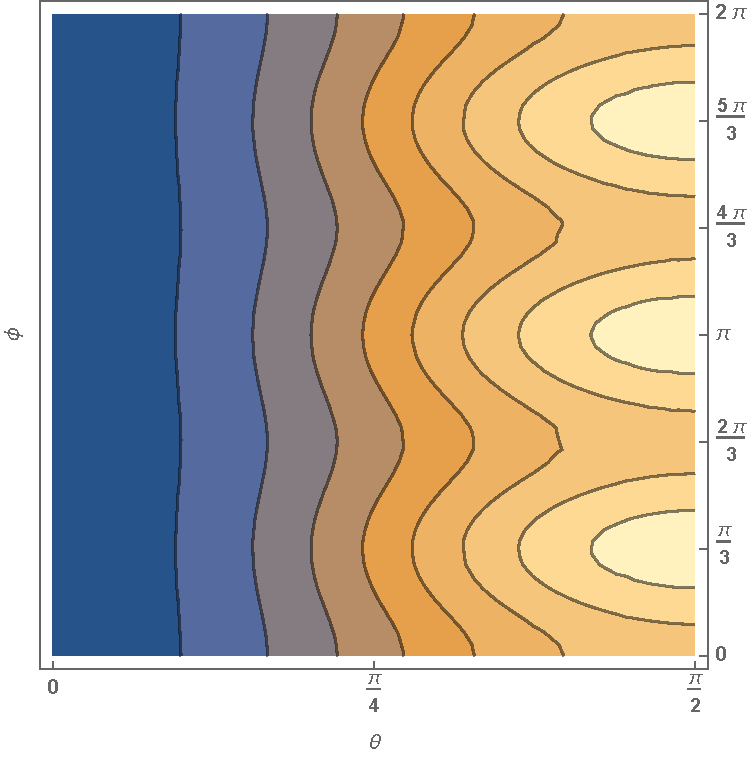
\includegraphics[width=0.60\linewidth]{potential.pdf}
	\caption{Potential surface for three identical particles. Symmetries due to translations and reflections are seen at $\phi = n\pi/3, \ (n = 1-5)$.}
	\label{fig:potential}
\end{figure*}

\subsection{Transformation of the Kinetic Energy Operator}\label{Appendix_2_2}
The kinetic energy operator of a particle with mass $\mu$ in a curvilinear coordinate system of $N$ dimensions is given by \cite{podolsky_1928}

\begin{equation}\label{eq:kinetic_e_op}
T = -\frac{1}{2\mu} \sum_{i=1}^{N} \sum_{j=1}^{N} \frac{1}{\sqrt{g}} \frac{\partial}{\partial q_i} \bigg(\sqrt{g} g^{ij} \frac{\partial}{\partial q_j}\bigg),
\end{equation}
where $g^{ij}$ is the inverse, or contravariant, metric tensor and $g$ is the determinant of the covariant metric tensor $g = \det(g_{ij}) \neq 0$. The metric tensor $g_{ij}$ describes the relationship between the set of curvilinear coordinates $\mathbf{q}$ and the set of regular Cartesian coordinates $\mathbf{x}$ through

\begin{equation}
g_{ij} = \sum_{\lambda = 1}^{N} \frac{\partial x_{\lambda}}{\partial q_{i}} \frac{\partial x_{\lambda}}{\partial q_{j}},
\end{equation}
where $x_{\lambda} = x_{\lambda}(q_1,\ldots,q_N)$. The metric is useful for generalizing the concept of distance to general curvilinear coordinate frames and hence maintaining the invariance of distance in different coordinate systems. Invariance of the square of the line element $d s^2$ under coordinate transformations can also be considered to define the metric itself, since

\begin{equation}
d s^2 = d\mathbf{x} \cdot d\mathbf{x} = \sum_{i,j}^{N} g_{ij}  d q_{i} d q_{j} = g.
\end{equation}
Here the displacement differential vector is given by

\begin{equation}
d\mathbf{x} = \frac{\partial \mathbf{x}}{\partial q_{i}} d q_{i},
\end{equation} 
where $\mathbf{x}$ is the position vector.

The transformation of interest for us is that from the mass weighted Jacobi coordinates $\mathbf{r}_k$ and $\mathbf{R}_k$ to a set of symmetric coordinates. Here we chose to work with one of the pair of the Jacobi coordinate sets $(i,j,k)=(1,2,3)$ and suppress the subscript. Since the three-body system has $N=6$ dimensions after separating out the centre-of-mass we collect the Cartesian components of the mass-weighted Jacobian vectors into the $6$-position

\begin{equation}
\mathbf{x} = 
\begin{pmatrix} 
\mathbf{r} \\
\mathbf{R} \\
\end{pmatrix} = 
\begin{pmatrix}
r_x \\
r_y \\
r_z \\
R_x \\
R_y \\
R_z\\
\end{pmatrix}.
\end{equation}

We start from the definition of the internal coordinates given in \Cref{eq:SW}. To describe how rotations of the body-fixed frame affects the derivatives in the space-fixed frame it is enough to consider infinitesimal rotations.  Let $d\mathbf{\Omega}$ be the angular displacement differential vector of the rotating axes $xyz$ with respect to the fixed axes $x'y'z'$

\begin{equation}
d\mathbf{\Omega} =
\begin{pmatrix}
d\Omega_x\\
d\Omega_y\\
d\Omega_z\\
\end{pmatrix}.
\end{equation}
Then the displacement differential vectors in the space-fixed frame transform like


\begin{subequations}
	\begin{align}
	d{\mathbf{r}}' &= d\mathbf{r} + d\mathbf{\Omega} \times \mathbf{r},\\
	d{\mathbf{R}}' &= d\mathbf{R} + d\mathbf{\Omega} \times \mathbf{R},
	\end{align}
\end{subequations}   
which is given explicitly by

\begin{align}
\begin{pmatrix}
d r'_x \\
d r'_y \\
d r'_z \\
d R'_x \\
d R'_y \\
d R'_z\\
\end{pmatrix} 
&= 
\begin{pmatrix*}[c]
\partial_{\rho} r_x & \partial_{\Theta} r_x & \partial_{\Theta} r_x & 0 & r_z & -r_y\\
\partial_{\rho} r_y & \partial_{\Theta} r_y & \partial_{\Theta} r_y & -r_z & 0 & r_x\\
\partial_{\rho} r_z & \partial_{\Theta} r_z & \partial_{\Theta} r_z & r_y & -r_x & 0\\
\partial_{\rho} R_x & \partial_{\Theta} R_x & \partial_{\Theta} R_x & 0 & R_z & -R_y\\
\partial_{\rho} R_y & \partial_{\Theta} R_y & \partial_{\Theta} R_y & -R_z & 0 & R_x\\
\partial_{\rho} R_z & \partial_{\Theta} R_z & \partial_{\Theta} R_z & R_y & -R_x & 0\\
\end{pmatrix*}
\begin{pmatrix}
d\rho\\
d\Theta\\
d\Phi\\
d\Omega_x\\
d\Omega_y\\
d\Omega_z\\
\end{pmatrix} \notag \\
&=
\begin{pmatrix*}[c]
\mathrm{cc} & \mathrm{-sc} & \mathrm{-cs} & 0 & 0 & \mathrm{ss}\\
\mathrm{-ss} & \mathrm{-cs} & \mathrm{-sc} & 0 & 0 & \mathrm{cc}\\
0 & 0 & 0 & \mathrm{-ss} & \mathrm{-cc} & 0\\
\mathrm{cs} & \mathrm{-ss} & \mathrm{cc} & 0 & 0 & \mathrm{-sc}\\
\mathrm{sc} & \mathrm{cc} & \mathrm{-ss} & 0 & 0 & \mathrm{cs}\\
0 & 0 & 0 & \mathrm{sc} & \mathrm{-cs} & 0\\
\end{pmatrix*}
\begin{pmatrix}
d\rho\\
\rho d\Theta\\
\rho d\Phi\\
\rho d\Omega_x\\
\rho d\Omega_y\\
\rho d\Omega_z\\
\end{pmatrix},\label{eq:matrix}
\end{align}
where the abbreviations are $\mathrm{cc} = \cos\Theta\cos\Phi$, $\mathrm{ss} = \sin\Theta\sin\Phi$, $\mathrm{cs} = \cos\Theta\sin\Phi$ and $\mathrm{sc} = \sin\Theta\cos\Phi$. In matrix notation \eqref{eq:matrix} may be expressed as

\begin{equation}
d\mathbf{x}' = \mathbf{A}d\mathbf{q},
\end{equation} 
in which      

\begin{equation}
d\mathbf{q} =
\begin{pmatrix}
d\rho\\
d\Theta\\
d\Phi\\
d\Omega_x\\
d\Omega_y\\
d\Omega_z\\
\end{pmatrix}.
\end{equation}
The squared line element $d s^2$ is then given by 

\begin{equation}
d s^2 = d\mathbf{x}' \cdot d\mathbf{x}' = d\mathbf{q}^{\mathrm{T}} \mathbf{A}^{\mathrm{T}} \mathbf{A}d\mathbf{q} = d\mathbf{q}^{\mathrm{T}} \mathbf{g} d\mathbf{q}.
\end{equation}
Here the metric tensor

\begin{equation}
\mathbf{g}=\mathbf{A}^{\mathrm{T}} \mathbf{A}=
\begin{pmatrix}
\mathbf{G} & \mathbf{C}\\
\mathbf{C}^\mathrm{T} & \mathbf{K}
\end{pmatrix}
\end{equation}
is partitioned into the submatrices $\mathbf{G}$, $\mathbf{K}$ and $\mathbf{C}$, which from \Cref{eq:matrix} are given by 

\begin{align}
\mathbf{G} &=
\begin{pmatrix}
1 & 0      & 0\\
0 & \rho^2 & 0\\
0 & 0      & \rho^2
\end{pmatrix},\\
\mathbf{K} &=
\rho^2
\begin{pmatrix}
\sin^2\Theta & 0            & 0\\
0            & \cos^2\Theta & 0\\
0            & 0            & 1
\end{pmatrix},\\
\intertext{and}
\mathbf{C} &=
-\rho^2\sin^2(2\Theta)
\begin{pmatrix}
0 & 0 & 0\\
0 & 0 & 0\\
0 & 0 & 1
\end{pmatrix},
\end{align}
respectively. The determinant of the metric tensor is then

\begin{align}
g &=
\mid\mathbf{g}\mid=
\begin{vmatrix}
\mathbf{G} & \mathbf{C}\\
\mathbf{C}^T & \mathbf{K}
\end{vmatrix}
=
\frac{\rho^{10}}{16}\sin^2(4\Theta)
\end{align}
and subsequently the square root of the metric reads
\begin{equation}
\sqrt{g}=\frac{\rho^5}{4}\sin(4\Theta).
\end{equation}
The inverse of the metric tensor $\mathbf{g}^{-1}$ is then given by

\begin{equation}
\mathbf{g}^{-1}=
\begin{pmatrix}
\mathbf{V} & \mathbf{W}\\
\mathbf{W}^\mathrm{T} & \mathbf{U}
\end{pmatrix},
\end{equation}
where the submatrices $\mathbf{V}$, $\mathbf{W}$ and $\mathbf{U}$ are given by

\begin{align}
\mathbf{V} &=
\begin{pmatrix}
1 & 0      & 0\\
0 & 1/\rho^2 & 0\\
0 & 0      & 1/\rho^2\cos^2(2\Theta)
\end{pmatrix},\\
\mathbf{U} &=
\frac{1}{\rho^2}
\begin{pmatrix}
1/\sin^2\Theta & 0            & 0\\
0            & 1/\cos^2\Theta & 0\\
0            & 0            & 1/\cos^2(2\Theta)
\end{pmatrix},\\
\intertext{and}
\mathbf{W} &=
\frac{\sin(2\Theta)}{\rho^2\cos^2(2\Theta)}
\begin{pmatrix}
0 & 0 & 0\\
0 & 0 & 0\\
0 & 0 & 1
\end{pmatrix},
\end{align}
respectively. Now, if the momentum vector is given by

\begin{equation}
\mathbf{p} = i 
\begin{pmatrix}
\partial/\partial q_1\\
\vdots\\
\partial/\partial q_N\\
\end{pmatrix},
\end{equation}
then we can express the kinetic energy operator given in \eqref{eq:kinetic_e_op} in terms of this vector and the metric

\begin{equation}\label{eq:T_SW}
\begin{aligned}
-T &= -\frac{1}{2\mu \sqrt{g}} \mathbf{p}^\mathrm{T} \sqrt{g} \mathbf{g}^{-1} \mathbf{p}\\
&= \frac{1}{2\mu \rho^5 \sin(4\Theta)}\Bigg[ \frac{\partial}{\partial \rho} \Bigg(\rho^5 \sin(4 \Theta) \frac{\partial}{\partial \rho}\Bigg) + \frac{\partial}{\partial \Theta}\Bigg(\rho^3\sin(4\Theta)\frac{\partial}{\partial\Theta}\Bigg)\\ &+\frac{\partial}{\partial\Phi}\Bigg(2\rho^3\tan(2\Theta)\frac{\partial}{\partial\Phi} + 2\tan^2(2\Theta)\cos(2\Theta)\frac{\partial}{\partial\Omega_z}\Bigg)\\
&+\frac{\partial}{\partial\Omega_x}\Bigg(4\rho^3\cot(\Theta)\cos(2\Theta)\frac{\partial}{\partial\Omega_x}\Bigg)\\
&+\frac{\partial}{\partial\Omega_y}\Bigg(4\rho^3\tan(2\Theta)\cos(2\Theta)\frac{\partial}{\partial\Omega_y}\Bigg)\\
&+\frac{\partial}{\partial\Omega_z}\Bigg(2\rho^3\tan^2(2\Theta)\frac{\partial}{\partial\Phi}+2\rho^3\tan(2\Theta)\frac{\partial}{\partial\Omega_z}\Bigg)\Bigg]\\
&=\frac{1}{2\mu\rho^5}\frac{\partial}{\partial\rho}\Bigg(\rho^5\frac{\partial}{\partial\rho}\Bigg) + \frac{1}{2\mu\rho^2}\Bigg[\frac{1}{\sin(4\Theta)}\frac{\partial}{\partial\Theta}\Bigg(\sin(4\Theta)\frac{\partial}{\partial\Theta}\Bigg)\\
&+\frac{1}{\cos^2(2\Theta)}\frac{\partial^2}{\partial\Phi^2} \Bigg]+\frac{1}{2\mu\rho^2}\Bigg[\frac{1}{\sin^2(\Theta)}\frac{\partial^2}{\partial\Omega^2_x} + \frac{1}{\cos^2(\Theta)}\frac{\partial^2}{\partial\Omega^2_y} + \frac{1}{\cos^2(2\Theta)}\frac{\partial^2}{\partial\Omega^2_z}\\
&+ \frac{2\sin(2\Theta)}{\cos^2(2\Theta)}\frac{\partial}{\partial\Phi}\frac{\partial}{\partial\Omega_z}\Bigg].
\end{aligned}
\end{equation}

To understand the last term in the kinetic energy operator we need to make a detour and discuss the spatial orientation of the triangle formed by the three particles in terms of Euler angles. However, for $J=0$ states this last term vanishes and then \Cref{eq:T_SW} reduces to the kinetic energy term in the Hamiltonian in \Cref{eq:hamiltonian_0}. 

As has been mentioned previously, we use the Euler angles $\alpha,\beta,\gamma$ to relate the body-fixed axes $xyz$ with the space-fixed axes $x'y'z'$. Any coordinate frame that coincides with the space-fixed frame can be made to coincide with the body-fixed frame as well by performing a series of three basic rotations (right-handed). There are several ways for defining the Euler angles; the convention used by Johnson \cite{Johnson_1983} is adopted here and the method is described in detail in \cite{arfken_weber_harris_2013}. If the line of nodes $\xi$ is the intersection of the planes $x'y'$ and $xy$, then $\alpha$ is the angle between the $y'$-axis and the line of nodes. The operational sequence is the following:

\begin{enumerate}[(i)]  
	\item First rotate the coordinates $x'y'z'$ counterclockwise through an angle $\alpha$ in the range $0 \leq \alpha < 2\pi$ about the $z'$-axis, using $\mathbf{S}_{\alpha}$, into the new coordinates $\bar{x}'\xi z'$.
	\item Then rotate the coordinates $\bar{x}' \xi z'$ counterclockwise through an angle $\beta$ $(0 \leq \beta \leq \pi)$ about the line of nodes, using $\mathbf{S}_{\beta}$, into the new coordinates $\bar{x} \xi z$.
	\item Finally rotate the coordinates $\bar{x} \xi z$ counterclockwise by an angle $\gamma$ $(0 \leq \gamma < 2\pi)$ about the $z$-axis (the former $z'$-axis) using $\mathbf{S}_{\gamma}$, into the body-fixed coordinates $xyz$.
\end{enumerate}   
The total rotation matrix is then the triple matrix product of the basic rotation matrices $\mathbf{S} = \mathbf{S}_{\alpha}\mathbf{S}_{\beta}\mathbf{S}_{\gamma}$, in which

\begin{equation}
\mathbf{S}_{\alpha}=
\begin{pmatrix}
\cos\alpha & \sin\alpha  & 0\\
-\sin\alpha & \cos\alpha & 0\\
0            & 0            & 1
\end{pmatrix},\\
\end{equation}

\begin{equation}
\mathbf{S}_{\beta}=
\begin{pmatrix}
\cos\beta & 0  & -\sin\beta\\
0 & 1 & 0\\
\sin\beta & 0  & \cos\beta
\end{pmatrix},\\
\end{equation}

\begin{equation}
\mathbf{S}_{\gamma}=
\begin{pmatrix}
\cos\gamma & \sin\gamma  & 0\\
-\sin\gamma & \cos\gamma & 0\\
0            & 0            & 1
\end{pmatrix},\\
\end{equation}
and

\begin{equation}
\mathbf{S}=
\begin{pmatrix}
\cos\gamma \cos\beta \cos\alpha -\sin\gamma \sin\alpha & \cos\gamma \cos\beta \sin\alpha \sin\gamma \cos\alpha  & -\cos\gamma \sin\beta\\
-\sin\gamma \cos\beta \cos\alpha -\cos\gamma \sin\alpha & \sin\gamma \cos\beta \sin\alpha +\cos\gamma \cos\alpha & \sin\gamma \sin\beta\\
\sin\beta \cos\alpha & \sin\beta \sin\alpha & \cos\beta
\end{pmatrix}.
\end{equation}
The Cartesian coordinates $\mathbf{x}$ and $\mathbf{x}'$ of a point $P$ in the two frames are thus related through

\begin{equation}
\mathbf{x} = \mathbf{S}\mathbf{x}'. 
\end{equation}
Now, the general angular displacement differential  $d\mathbf{\Omega}$ can be considered to consist of three consecutive infinitesimal rotations where $d\Omega_{\alpha} = d\alpha$, $d\Omega_{\beta} = d\beta$ and $d\Omega_{\gamma} = d\gamma$. The vector $d\mathbf{\Omega}$ can be obtained as the sum of three different angular displacement differential vectors; $d\mathbf{\Omega_{\alpha}}$ is along the space-fixed $z'$-axis, $d\mathbf{\Omega_{\beta}}$ is along the line of nodes and $d\mathbf{\Omega_{\gamma}}$ is along the body-fixed $z$-axis \cite{goldstein_poole_safko_2000}. Since $d\mathbf{\Omega_{\alpha}}$ is along the $z'$-axis, its components are obtained by applying the total rotation matrix. Thus, if the total rotation matrix is written

\begin{equation}
\mathbf{S} = [\mathbf{S}_1 \quad \mathbf{S}_2 \quad \mathbf{S}_3],
\end{equation}
then the body-fixed displacement differential angles $d\mathbf{\Omega}_{\alpha}$ are related to the Euler angles through

\begin{equation}
(\mathbf{\Omega}_{\alpha})_{\mathbf{x}} = \mathbf{S}_3 d\alpha= 
\begin{pmatrix}
-\sin\beta \cos\gamma \\
\sin\beta \sin\gamma \\
\cos\beta
\end{pmatrix} d\alpha.
\end{equation}
Next, because $d\mathbf{\Omega_{\beta}}$ is along the line of nodes, we only need to apply the last transformation $\mathbf{S}_{\gamma}$ to retrieve

\begin{equation}
(\mathbf{\Omega}_{\beta})_{\mathbf{x}} = \mathbf{S}_{\gamma_2} d\beta= 
\begin{pmatrix}
\sin\gamma \\
\cos\gamma \\
0
\end{pmatrix} d\beta.
\end{equation}
No transformation is needed for $d\mathbf{\Omega_{\gamma}}$ since it is already directed along the body-fixed $z$-axis. The transformations are finally summarized into the total transformation matrix, which relates the body-fixed infinitesimal rotations to the Euler angles through

\begin{equation}
\begin{pmatrix}
d\Omega_x\\
d\Omega_y\\
d\Omega_z
\end{pmatrix}
=
\tilde{\mathbf{S}}\begin{pmatrix}
d\alpha\\
d\beta\\
d\gamma
\end{pmatrix},
\end{equation}
where

\begin{equation}\label{eq:S_matrix}
\tilde{\mathbf{S}}=
\begin{pmatrix}
-\sin\beta\cos\gamma & \sin\gamma & 0\\
\sin\beta\sin\gamma  & \cos\gamma & 0\\
\cos\beta 			 & 0          & 1
\end{pmatrix}.
\end{equation}
Thus, a transformation of coordinates

\begin{equation}
d\mathbf{q} =
\begin{pmatrix}
d\rho\\
d\Theta\\
d\Phi\\
d\Omega_x\\
d\Omega_y\\
d\Omega_z\\
\end{pmatrix}
\longrightarrow
d\mathbf{q}' =
\begin{pmatrix}
d\rho\\
d\Theta\\
d\Phi\\
d\alpha\\
d\beta\\
d\gamma\\
\end{pmatrix}
\end{equation}
corresponds to a transformation of the metric, which is easily derived from the squared line element, where

\begin{equation}
d s^2 = d \mathbf{q}^{\mathrm{T}}\mathbf{g}d \mathbf{q} = (d \mathbf{q}')^\mathrm{T}\mathbf{g}'d\mathbf{q}'.
\end{equation}
The metric thus transforms as 

\begin{equation}
\mathbf{g}'=\mathbf{B}^{\mathrm{T}}\mathbf{g}\mathbf{B},
\end{equation}
in which

\begin{equation}
\mathbf{B} = 
\begin{pmatrix}
\mathbf{I} & 0\\
0      & \tilde{\mathbf{S}}
\end{pmatrix}.
\end{equation}
Subsequently, the square root of the determinant transforms into

\begin{equation}
g'^{1/2}=(\mid\mathbf{B}\mid^2 \mid\mathbf{g}\mid)^{1/2} = (\mid\tilde{\mathbf{S}}\mid^2 \mid\mathbf{g}\mid)^{1/2}
= \frac{\rho^5}{4}\sin(4\Theta)\sin\beta.
\end{equation}
Since a general curvilinear coordinate system of $N$ dimensions has a volume element

\begin{equation}
d ^Nv = g^{1/2}\prod_{i=1}^{N} d q_i,
\end{equation}
the sought volume element is  

\begin{equation}
d^6v = g^{1/2}\prod_{i=1}^{6} d q_i = \frac{\rho^5}{4}\sin(4\Theta)\sin\beta \,d\rho \,d\Theta \, d\Phi \, d\alpha \,d\beta \,d\gamma.
\end{equation}
Lastly, to produce a representation of the entire internal configuration
space that is unbiased by the particular choice of the three Jacobi coordinate sets, we follow Kuppermann's mapping procedure \cite{KUPPERMANN1975374} and make the modification of the internal angles described in \Cref{eq:SW_trans}. Now, define

\begin{equation}
\mathbf{P} = 
-i
\begin{pmatrix}
\partial/\partial\rho\\
\partial/\partial\theta\\
\partial/\partial\phi
\end{pmatrix}
=
\begin{pmatrix}
P_{\rho}\\
P_{\theta}\\
P_{\phi}
\end{pmatrix}
\end{equation}
and

\begin{equation}\label{eq:J_vector}
\mathbf{J} = 
-i
\begin{pmatrix}
\partial/\partial\Omega_x\\
\partial/\partial\Omega_y\\
\partial/\partial\Omega_z
\end{pmatrix}
=
\begin{pmatrix}
J_x\\
J_y\\
J_z
\end{pmatrix},
\end{equation}
where the operators $J_x$, $J_y$ , and $J_z$ are the total angular momentum operators in the body-fixed frame, which can be expressed in terms of the Euler angle coordinates by the relation

\begin{equation}
\begin{pmatrix}
J_x\\
J_y\\
J_z
\end{pmatrix} =
\begin{pmatrix}
-\cos\gamma/\sin\beta & \sin\gamma & \cot\beta \cos\gamma\\
\sin\gamma/\sin\beta & \cos\gamma & -\cot\beta \sin\gamma\\
0 & 0 & 1
\end{pmatrix}
\begin{pmatrix}
P_{\alpha}\\
P_{\beta}\\
P_{\gamma}
\end{pmatrix}.
\end{equation} 
This can be shown using the chain rule for partial differentiation

\begin{equation}
P_{\sigma} = \sum_{\lambda} \frac{\partial \Omega_{\lambda}}{\partial \sigma} J_{\lambda},
\end{equation}
where $\sigma = (\alpha,\beta,\gamma)$ and $\lambda = (x,y,z)$. The partial derivatives are calculated using the inverse of \eqref{eq:S_matrix}, which is given by

\begin{equation}
\tilde{\mathbf{S}}^{-1}=
\begin{pmatrix}
-\cos\gamma/\sin\beta & \sin\gamma/\sin\beta & 0\\
\sin\gamma  & \cos\gamma & 0\\
\cot\beta \cos\gamma  & -\cot\beta \sin\gamma  & 1
\end{pmatrix}.
\end{equation}
Now, using the relations

\begin{equation}
\begin{aligned}
&\sin 4\Theta   =\sin 2\theta\\
&\cos^2 2\Theta =\sin^2 \theta\\
&\sin^2 2\Theta =\cos^2 \theta\\
&\cos^2\Theta    =\frac{1}{2}(1+\sin\theta)\\
&\sin^2\Theta    =\frac{1}{2}(1-\sin\theta)
\end{aligned}
\end{equation}
in conjunction with \eqref{eq:J_vector}, the kinetic energy operator \eqref{eq:T_SW} becomes

\begin{equation}
\begin{aligned}
T &=-\frac{1}{2\mu}\Bigg[\frac{1}{\rho^5}\frac{\partial}{\partial\rho}\rho^5\frac{\partial}{\partial\rho} + \frac{4}{\rho^2}\Bigg(\frac{1}{\sin 2\theta}\frac{\partial}{\partial\theta}\sin 2\theta\frac{\partial}{\partial\theta} +\frac{1}{\sin^2 \theta}\frac{\partial^2}{\partial\phi^2} \Bigg)\Bigg]\\ &-\frac{1}{\mu\rho^2}\Bigg[\frac{J^2_x}{(1-\sin\theta)} + \frac{J^2_y}{(1+\sin\theta)} +\frac{J^2_z}{2\sin^2\theta}\Bigg]+ \frac{4i\cos\theta J_z}{2\mu\rho^2\sin^2\theta}\frac{\partial}{\partial\phi},
\end{aligned}
\end{equation}
with the corresponding volume element

\begin{equation}
d^6 v = \frac{1}{8}\rho^5 \sin\theta\cos\theta\sin\beta \, d\rho \, d\theta \, d\phi \, d\alpha \, d\beta \, d\gamma.
\end{equation}
If we only consider $J=0$ states, the Hamiltonian reduces to 

\begin{equation}
H_{0} = -\frac{1}{2 \mu} \Bigg[ \frac{1}{\rho^{5}} \frac{\partial}{\partial \rho} \rho^{5} \frac{\partial}{\partial \rho} + \frac{4}{\rho^{2}}\bigg( \frac{1}{\sin 2\theta} \frac{\partial}{\partial \theta} \sin 2\theta \frac{\partial}{\partial \theta} + \frac{1}{\sin^{2}\theta} \frac{\partial^{2}}{\partial \phi^{2}} \bigg) \Bigg] + V(\rho, \theta, \phi).\label{eq:hamiltonian_0}
\end{equation}
By rescaling the wavefunction $\psi = \rho^{5/2} \Psi$ the Schr{\"o}dinger equation becomes

\begin{equation}
H \psi = E \psi,
\end{equation}
where the transformed Hamiltonian operator is given by

\begin{equation}
H = \rho^{5/2}H_{0} \rho^{-5/2}. 
\end{equation}
This transformation removes the first derivative in the hyperradial kinetic energy operator and we get the final expression for the Hamiltonian

\begin{align}
H &= -\frac{\hbar^{2}}{2 \mu} \Bigg[ -\frac{15}{4} \frac{1}{\rho^{2}} + \frac{\partial^{2}}{\partial \rho^{2}}+ \frac{4}{\rho^{2}}\bigg( \frac{1}{\sin 2\theta} \frac{\partial}{\partial \theta} \sin 2\theta \frac{\partial}{\partial \theta} + \frac{1}{\sin^{2}\theta} \frac{\partial^{2}}{\partial \phi^{2}} \bigg) \Bigg] + V(\rho, \theta, \phi)\\
&= -\frac{\hbar^{2}}{2 \mu}\frac{\partial^2}{\partial \rho^2} + \frac{\hbar^{2}}{2 \mu \rho^{2} } \Bigg(\Lambda^2 + \frac{15}{4}\Bigg)+ V(\rho, \theta, \phi),
\end{align}
where $\Lambda^2$ is the squared grand angular momentum operator, which is given by

\begin{equation}
\Lambda^2 = -\frac{4}{\sin 2\theta} \frac{\partial}{\partial \theta} \sin 2\theta \frac{\partial}{\partial \theta} - \frac{4}{\sin^{2}\theta} \frac{\partial^{2}}{\partial \phi^{2}}.
\end{equation}   